\documentclass{beamer}
\usetheme{Antibes}

% removes navigation icons
\setbeamertemplate{navigation symbols}{}

\usepackage[utf8]{inputenc}
\usepackage{hyperref}
\usepackage{framed}
\usepackage{graphicx}
\usepackage{color}
\usepackage{cite}

\newcommand{\remove}[1]{}
%\newcomand{\mynote}[1]{}

\title{Identificação de elementos em documentos HTML baseado em estruturas semelhantes}
\author[Iam Jabour]{Iam Jabour \\ Orientador: Eduardo Laber \\ Co-orientador: Raúl Rentería}
\institute[PUC-Rio]{
  Pontifícia Universidade Católica do Rio de Janeiro \\
}
\date{27 de Janeiro 2010}

\newenvironment{my_itemize}{
\begin{itemize}
  \setlength{\itemsep}{5pt}
  \setlength{\parskip}{2pt}
  \setlength{\parsep}{3pt}
}{\end{itemize}}


\begin{document}

\begin{frame}
  \titlepage
\end{frame}

\AtBeginSubsection[]{
  \begin{frame}
    \frametitle{Sumário}

    \tableofcontents[currentsubsection]
  \end{frame}
}


\section{Introdução}

\subsection{Extração de informação da WEB}
\begin{frame}
\frametitle{Por que minerar a Web?}

  \begin{my_itemize}
  \item Fonte de informação em constante renovação
  \item Informação atualizada
  \item Demora na absorção de padrões e normas
  \end{my_itemize}
\end{frame}

\subsection{Tarefas de identificação e extração}

\begin{frame}
\frametitle{Tarefas de identificação e extração de informação da Web}
  \begin{my_itemize}

    \item[-] {\bf Extração de \textit{templates}}:
    limpar o documento, diminuindo a quantidade de informação não relevante 


    \item[-] {\bf Identificação de notícias}: identificar e extrair
    somente o texto da notícia para facilitar seu processamento 
\only<1>{
    \item[-] {\bf Extração de tabelas}:
    entender as informações apresentadas em tabelas
}
\only<2>{
    \item[-] \alert{{\bf Extração de tabelas}:
    entender as informações apresentadas em tabelas}
}

\only<1>{
    \item[-] {\bf Extração de itens em sites de comércio eletrônico}:
    recuperar as informações de itens em sites de comércio eletrônico
}
\only<2>{
    \item[-] \alert{{\bf Extração de itens em sites de comércio eletrônico}:
    recuperar as informações de itens em sites de comércio eletrônico}
}

  \end{my_itemize}
\end{frame}

\subsection{Extração de tabelas}

\begin{frame}
\frametitle{Entendendo a tarefa}%[allowframebreaks]
~\cite{Pinto2003} define 5 níveis de problemas na tarefa de extração de
tabelas:

  \begin{my_itemize}
\only<1>{
    \item[1] Localizar a tabela
}

\only<2>{
    \item[1] \alert{Localizar a tabela}
}
    \item[2] Identificar a posição das linhas e seus tipos
    \item[3] Identificar a posição das colunas e seus tipos
    \item[4] Rotular cada celula como dado ou legenda
    \item[5] Associar celulas de dados com sua legenda correspondente
  \end{my_itemize}
\end{frame}

\begin{frame}
\frametitle{Motivação}
  \begin{my_itemize}
    \item Importância de dados apresentados em tabelas
    \item Uso errado da \textit{tag} table por programadores
  \end{my_itemize}
\end{frame}

\begin{frame}
\frametitle{O que é uma tabela?}
    \begin{my_itemize}
      \item Tabela genuína: apresenta informações de forma tabular, onde o conteúdo de uma linha ou coluna tem o mesmo significado
    \end{my_itemize}

\begin{figure}[h]
  \center
  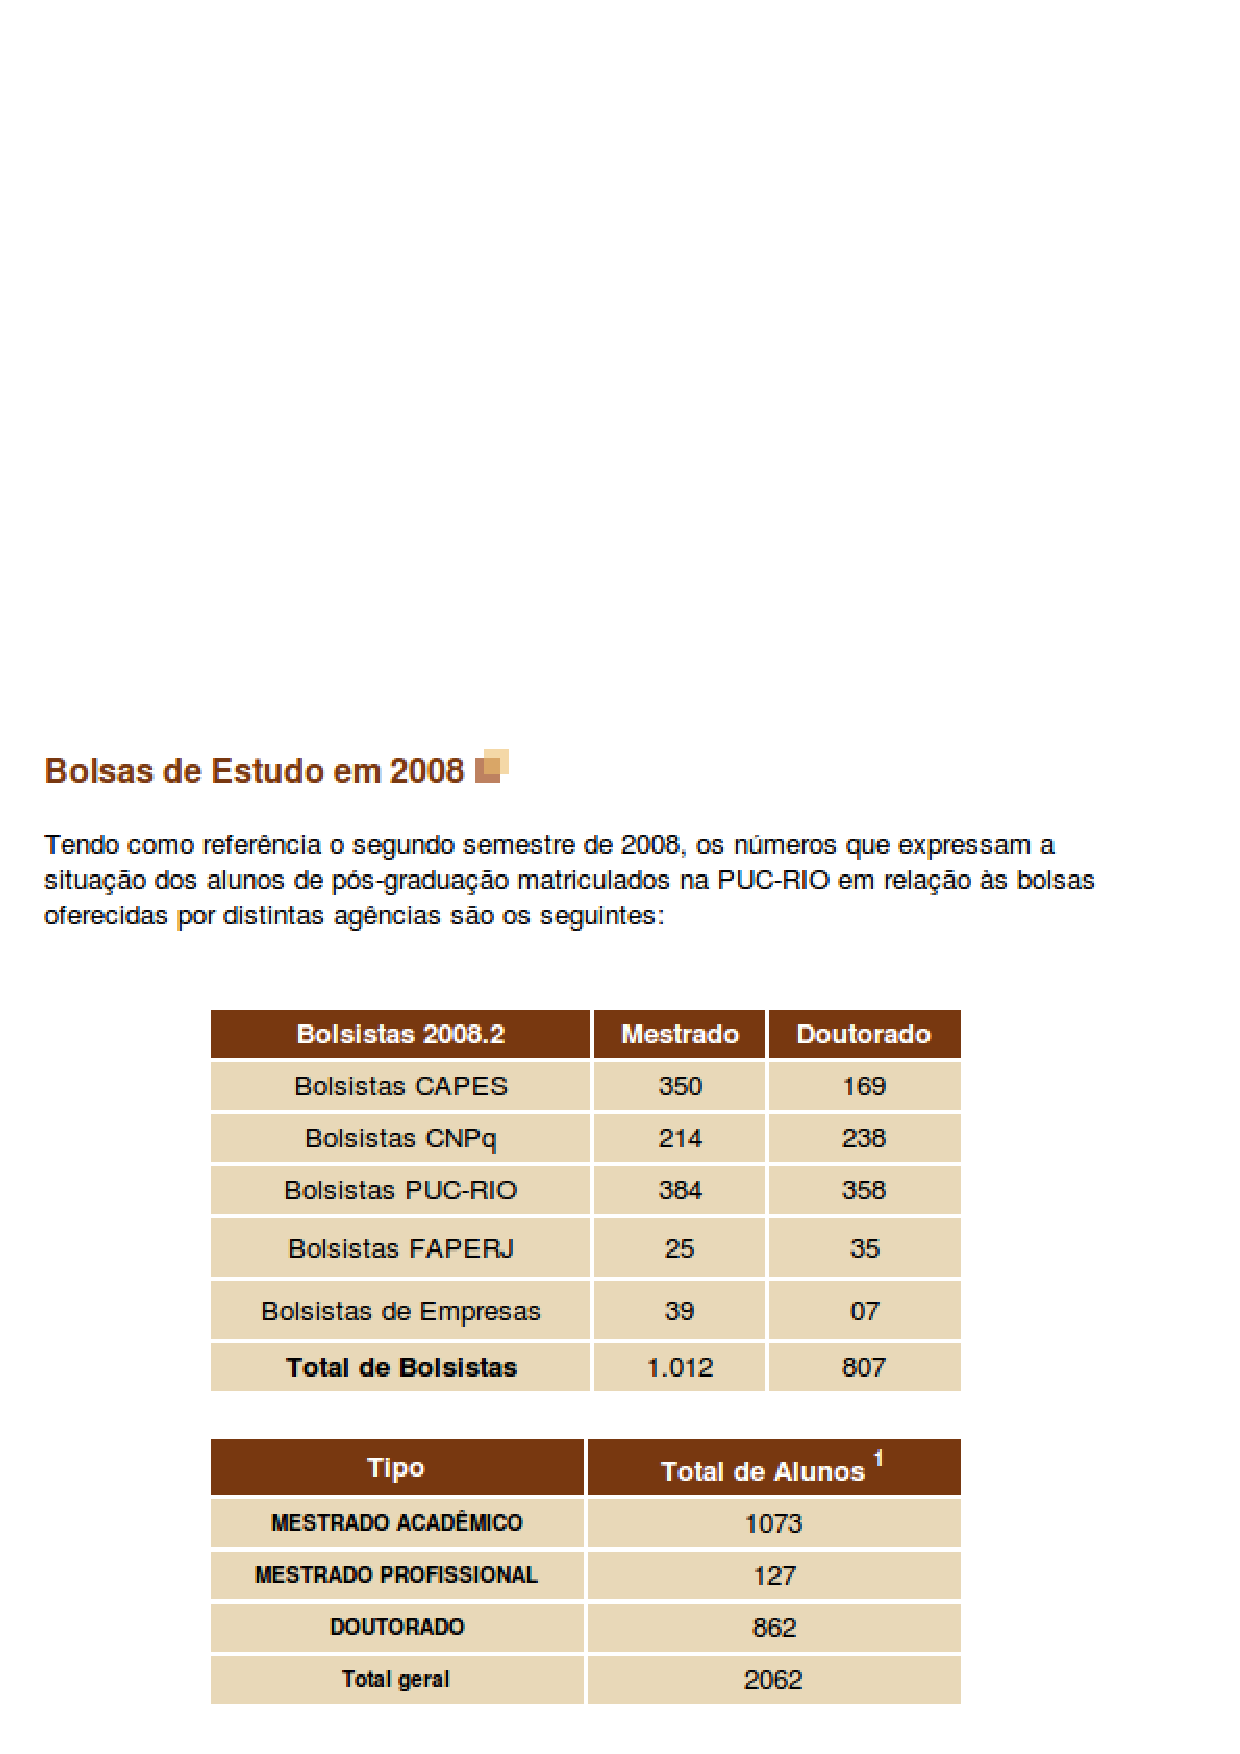
\includegraphics[scale=0.25]{img/table}
  \caption{retirado de: www.puc-rio.br/ensinopesq/ccpg/bolsas.html}
\end{figure}

\end{frame}


\begin{frame}
\frametitle{Trabalhos Relacionados}

  \begin{my_itemize}
    \item[-] ~\cite{Pinto2003}: Aborda o problema em texto puro, modela
    de forma a poder utilizar um {\it Conditional Random Fields} para resolver o problema de identificar linhas e determinar seus tipos.

\pause
   \item[-] ~\cite{Krupl2006}: Aborda o problema de forma visual, procurando blocos que podem ser tabelas (button-up).

\pause
   \item[-] ~\cite{Wang2002}: Aborda o problema de forma estrutural e textual, com features de estrutura (uso de tags), content (tipo de dados) e words (palavras chaves) utiliza técnicas de aprendizado de máquina para criar um classificador de tabelas genuínas.

  \end{my_itemize}

\end{frame}


\subsection{Extração de itens em sites de comércio eletrônico}
\begin{frame}
\frametitle{Entendendo a tarefa}
Extrair as informações contidas nos itens apresentados por sites de comércio eletrônico.

\begin{figure}[h!]
    \center
    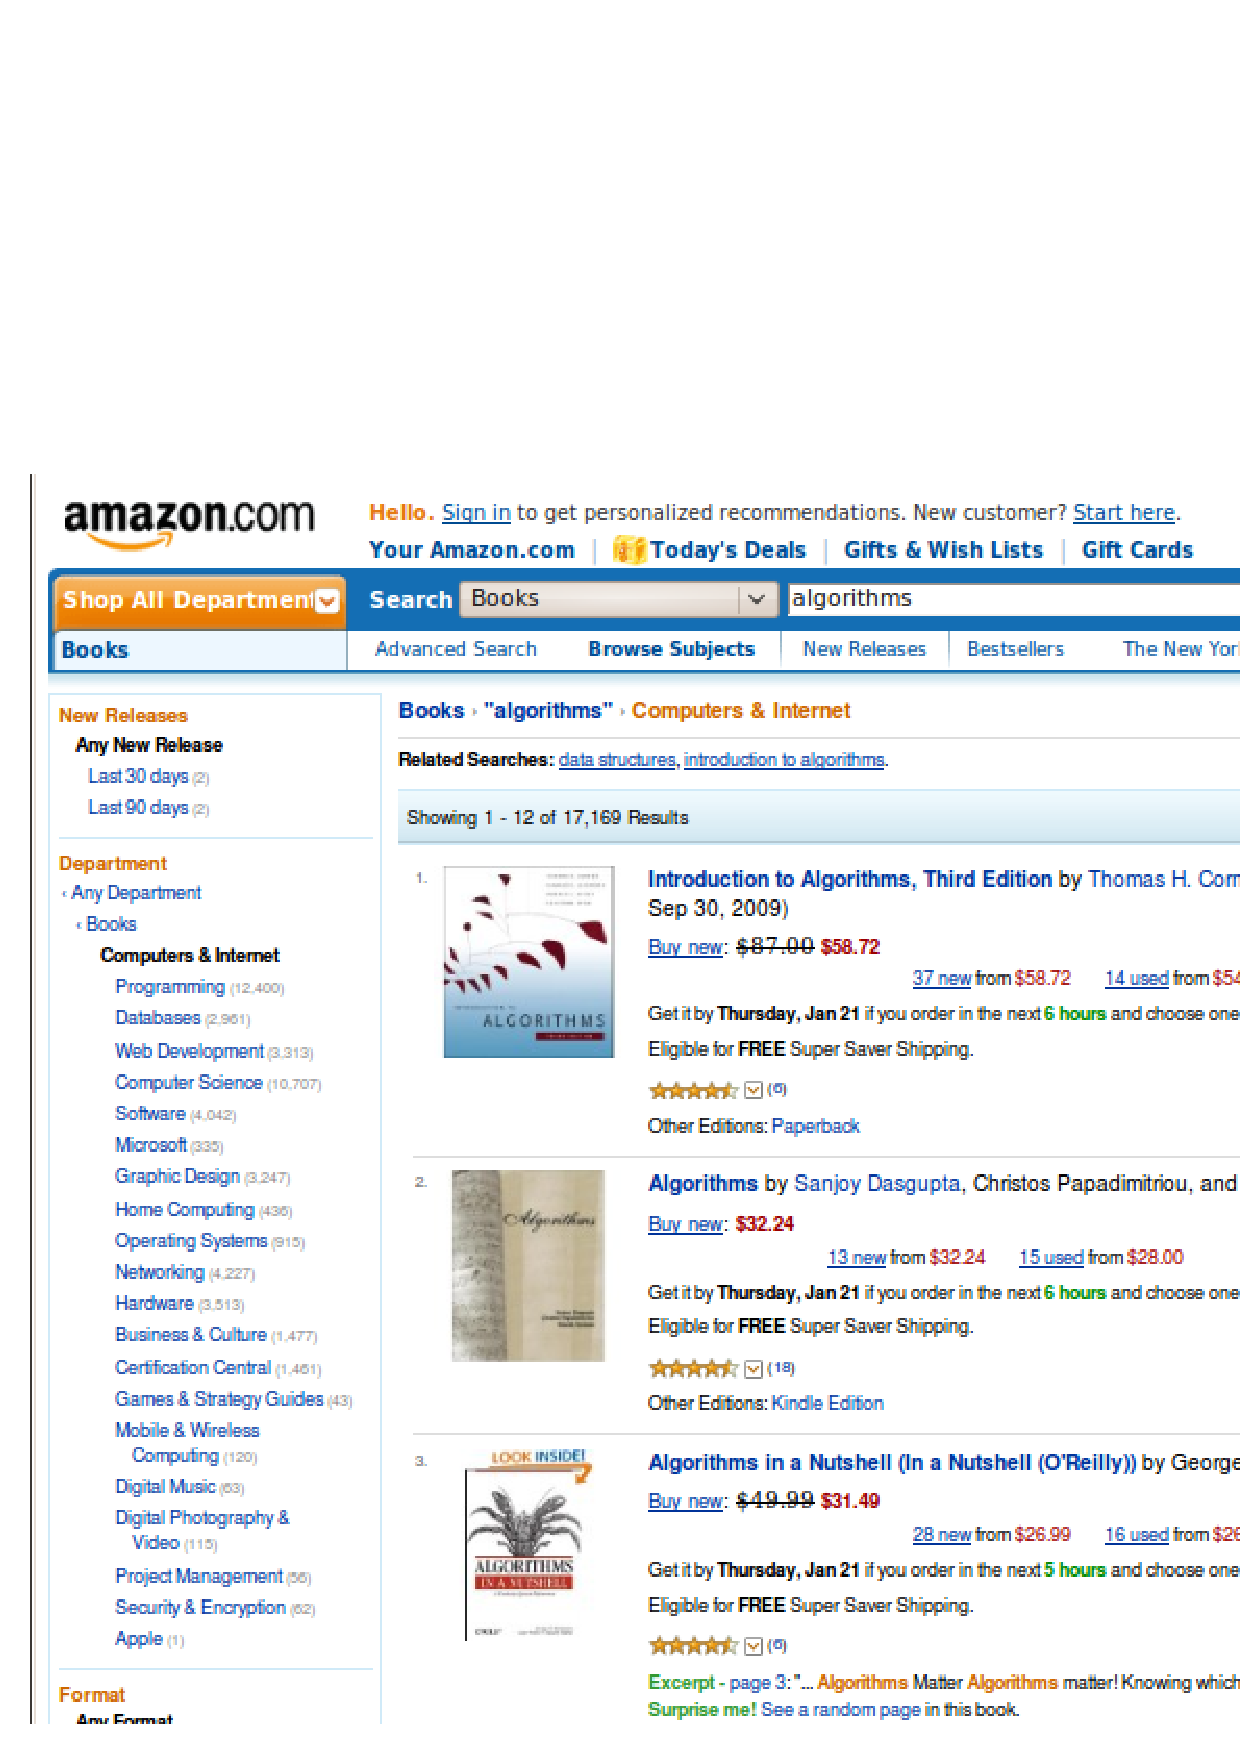
\includegraphics[scale=0.25]{img/ce}
\end{figure}

\end{frame}

\begin{frame}
\frametitle{Motivação}
    \begin{my_itemize}
    \item Capacidade de gerar consultas e buscas dos itens
    \item Capacidade de gerar comparações entre diferentes sites
    \item Agregar informações sobre preço e disponibilidade
    \end{my_itemize}
\end{frame}

\section{Proposta}

\subsection{Motivação e Abordagem}
\begin{frame}
\frametitle{Motivação}
  \begin{my_itemize}
    \item Estudar:
    \begin{my_itemize}
      \item Estrutura da árvore HTML em busca de semelhanças estruturais
    \end{my_itemize}

\only<1->{
    \item Para:
}
    \begin{my_itemize}

\only<1-2>{
      \item[-] Identificar tabelas
      \item[-] Identificar itens
}

\only<3->{
      \item[-] \alert{Identificar tabelas}
      \item[-] \alert{Identificar itens}
}

\only<1->{
      \item[-] Identificar template
}

\only<2->{
      \item[-] \alert{Identificar estruturas em geral}
}

    \end{my_itemize}
  
  \only<4->{
    \item Utilizando:
  Somente as informações contidas na estrutura HTML, sem
  renderizar ou utilizar qualquer tipo de análise semântica do texto
}

  \end{my_itemize}
\end{frame}

\begin{frame}
\frametitle{Por que utilizar a estrutura?}

  \begin{my_itemize}
  \item Informação semi-estruturada
  \item Velocidade
  \pause
  \item Existência do trabalho de ~\cite{Zhai2005} que utiliza uma árvore
  gerada a partir da página HTML para identificar listas e tabelas,
  denominado data records
    \begin{my_itemize}
    \item[-] Utiliza uma árvore que apresenta as mesmas
    características da árvore gerada a partir da estrutura do HTML
    \item[-] Não apresenta resultados da técnica para tarefas isoladas como
    identificação de tabela ou identificação de itens
    \end{my_itemize}
  \end{my_itemize}

\end{frame}

\begin{frame}[allowframebreaks]
\frametitle{Abordagem}
  \begin{figure}[h]
    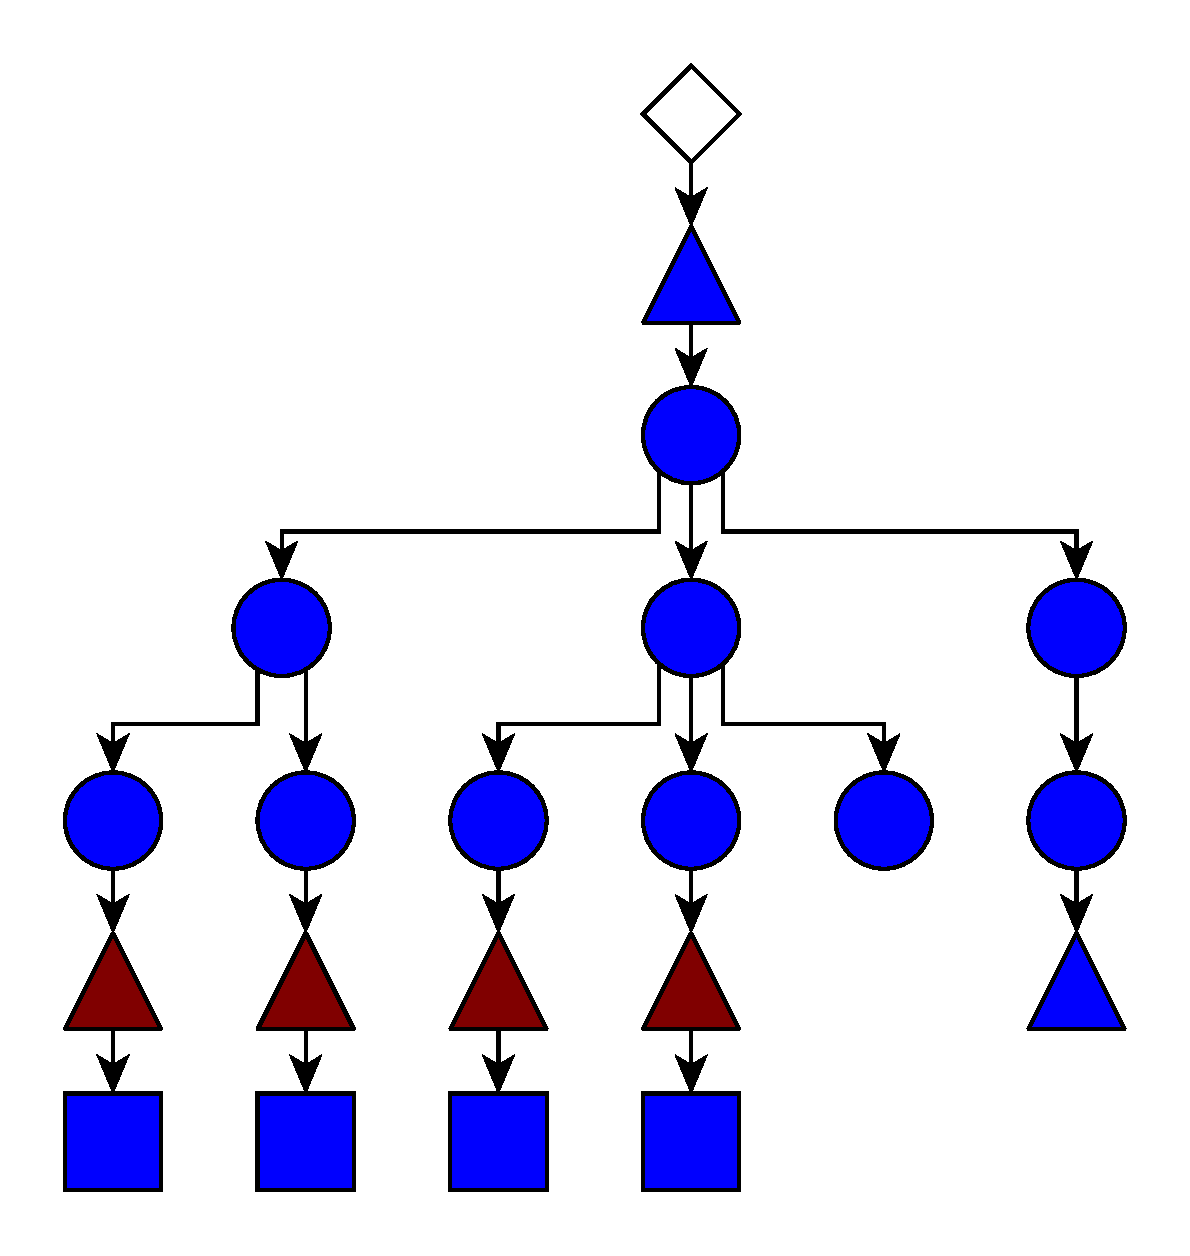
\includegraphics[scale=0.25]{img/tree0}
    \caption{Árvore HTML, subárvores vermelhas têm a mesma estrutura}
  \end{figure}

\newpage

  \begin{figure}[h]
    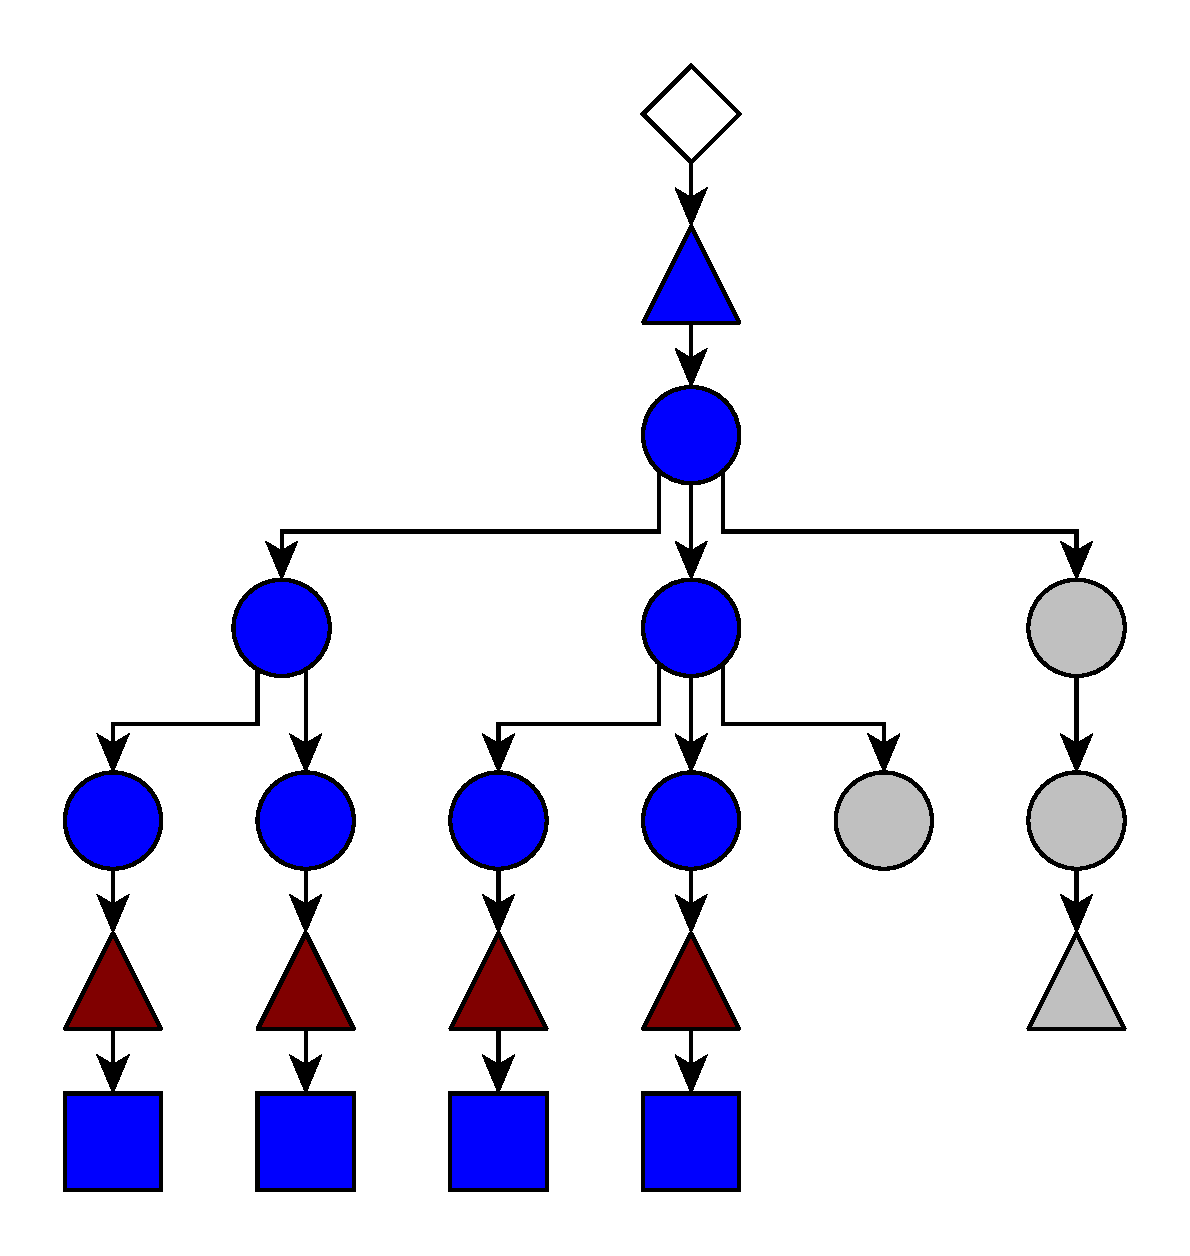
\includegraphics[scale=0.25]{img/tree1}
    \caption{Árvore que apresenta a mesma subestrutura, tipicamente listas e tabelas}
  \end{figure}

\newpage

  \begin{figure}[h]
    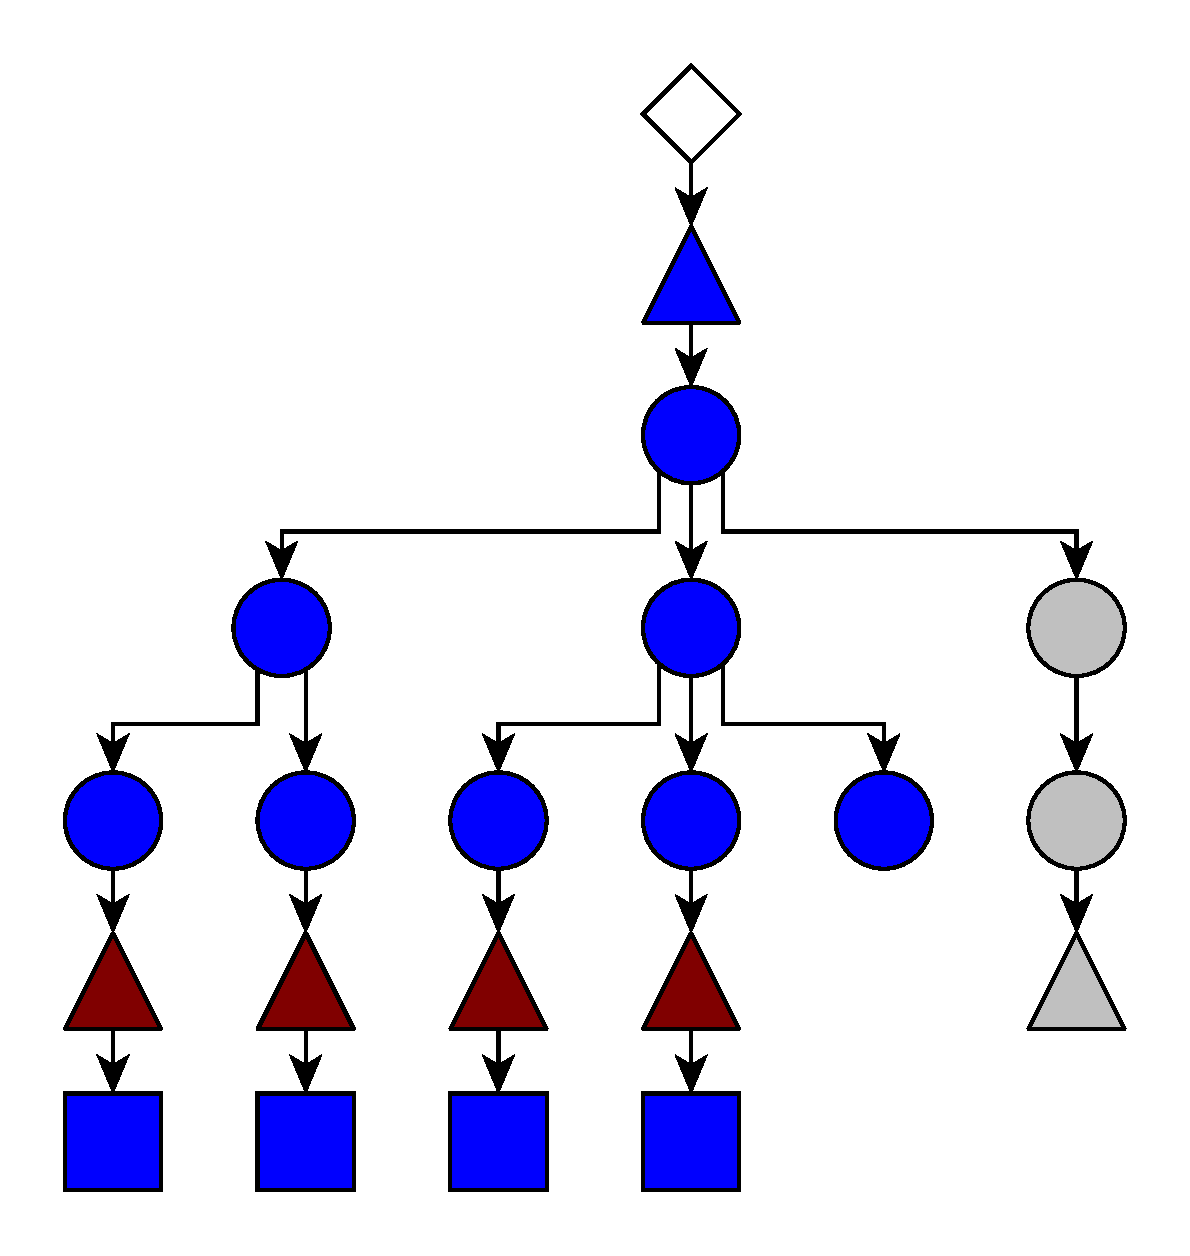
\includegraphics[scale=0.25]{img/tree2}
    \caption{Árvore que apresenta subestrutura semelhante}
  \end{figure}

\newpage

  \begin{figure}[h]
    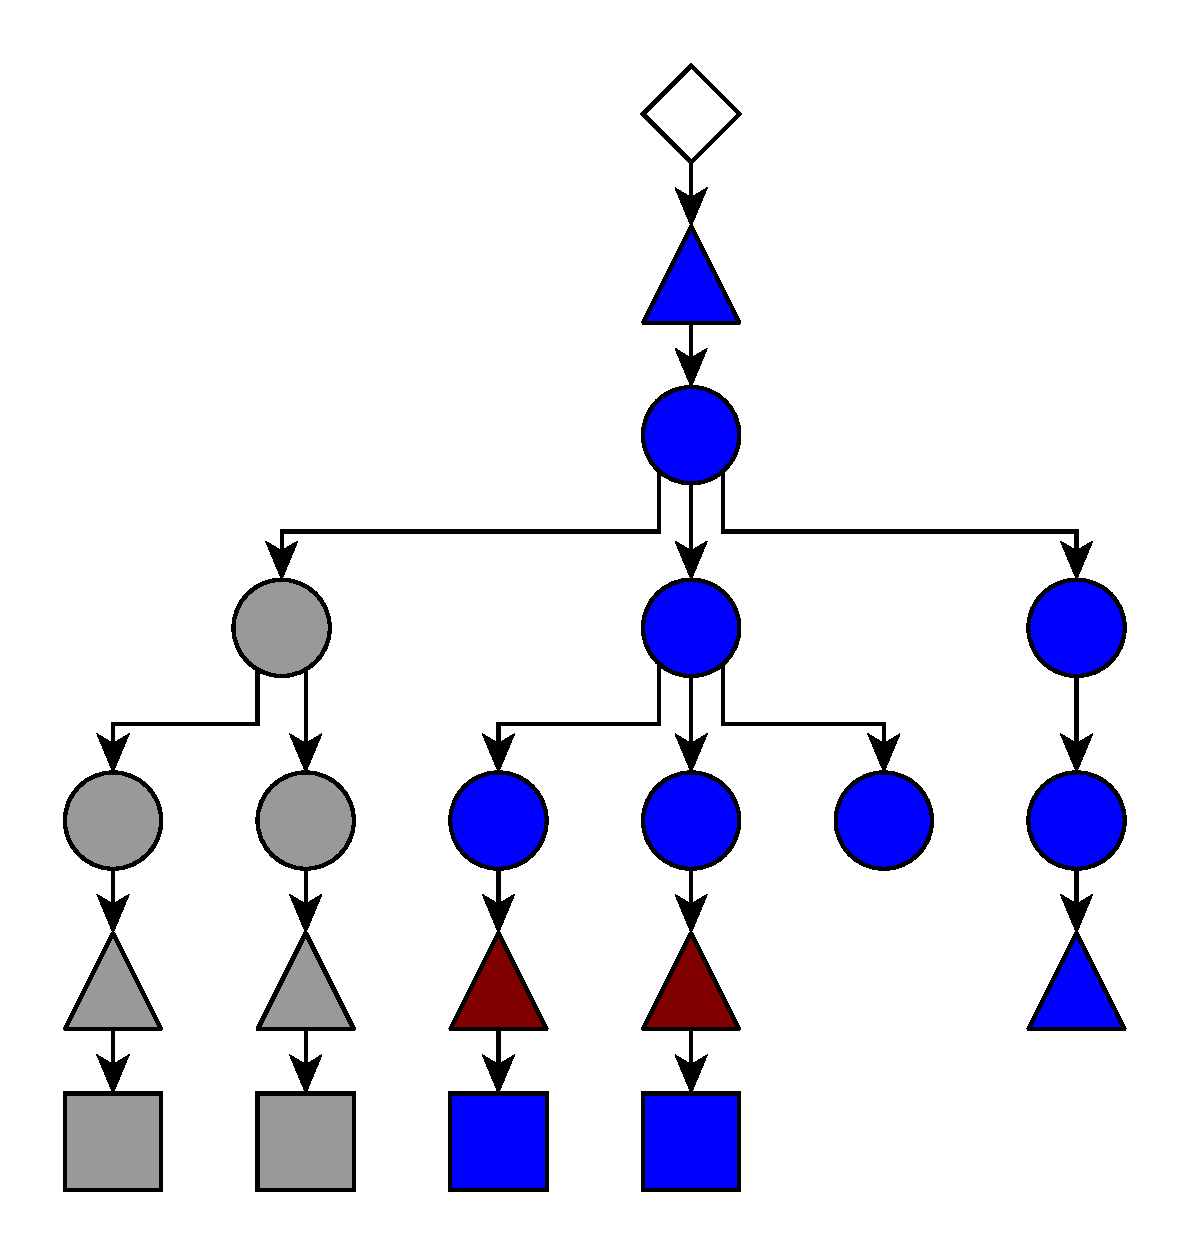
\includegraphics[scale=0.25]{img/tree3}
    \caption{Árvore que não contem semelhança em sua estrutura}
  \end{figure}

\end{frame}

\subsection{Andamento}

\begin{frame}
  \frametitle{Ambiente de experimentação}
  \begin{my_itemize}

    \item Construção de um ambiente que possibilite:
    \only<3->{\checkmark}

    \begin{my_itemize}
      \item[-] Realizar experimentos rápidos
      \item[-] Realizar experimentos com diferentes tarefas
      \pause
      \item[-] Utilizar diferentes corpus
      \item[-] Utilizar diferentes métricas
    \end{my_itemize}
  \end{my_itemize}

\end{frame}

\begin{frame}
\frametitle{Modelo do ambiente de experimentação}
\begin{center}
  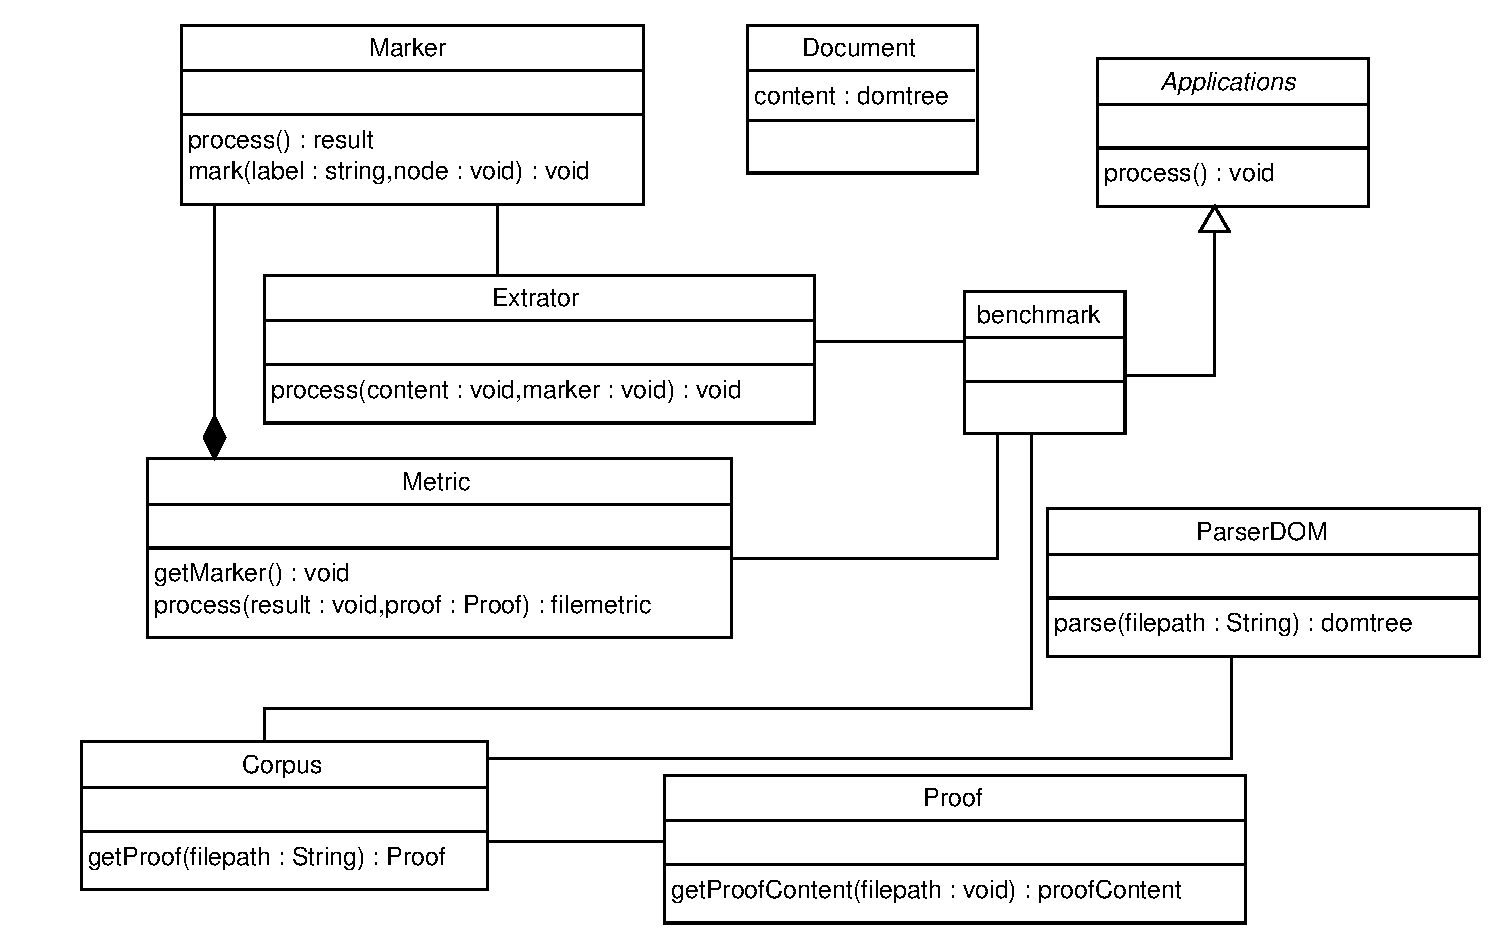
\includegraphics[scale=0.43]{img/classes}
\end{center}
\end{frame}

\begin{frame}
\frametitle{Corpora}
  \begin{my_itemize}
    \item Corpus para a tarefa de identificação de tabelas
    \begin{my_itemize}
      \item Corpus utilizando no trabalho de ~\cite{Wang2002}
      \item 1.392 documentos HTML de 200 web sites
      \item 14.609 \it{tags table}
      \item 11.477 tabelas internas
      \item 1.740 tabelas genuínas
    \end{my_itemize}
\pause

    \item Corpus para a tarefa de identificação de itens em sites de
    comércio elentrônico
    \begin{my_itemize}
      \item Será construido com documentos de pelo menos 20 web sites
      \item Conterá pelo menos 2.000 documentos, 100 de cada web site
    \end{my_itemize}
    
  \end{my_itemize}

\end{frame}


\begin{frame}
  \frametitle{Identificação de tabela}
  \begin{my_itemize}
   \item Dados estatísticos em 100 documentos
   \begin{my_itemize}
   \item Número de tabelas (\textit{tag table}): 1070
   \item Número de tabelas internas: 841 
   \item Número de tabelas genuínas: 130
   \end{my_itemize}

\pause
   \item Heurísticas existentes
   \begin{my_itemize}
   \item Regra básica: apenas verifica a semelhança entre os filhos no nó table
   \item Regra específica: Após aplicar a regra básica verifica se
   existem pelo menos duas colunas que contêm informação nessa tabela.
   Lista não devem ser marcadas como tabela.

   \end{my_itemize}
  \end{my_itemize}
\end{frame}

\begin{frame}
\frametitle{Resultados obtidos}
  \begin{center}
  \small{
  \begin{tabular}{| c | c | c | c |}
    \hline
    Regra & Recall & Precision & F-measure \\ \hline
    todas as tabelas & 1 & 0.121 & 0.215 \\ \hline
    tabelas internas & 0.976 & 0.151 & 0.261 \\ \hline
    regra básica & 0.923 & 0.264 & 0.410 \\ \hline
    regra avançada & 0.800 & 0.707 & 0.750 \\ \hline
  \end{tabular}
}
  \end{center}

\end{frame}

\subsection{Cronograma}

\begin{frame}
  \frametitle{Cronograma}
  \begin{center}
  \small{
  \begin{tabular}{| c | p{8cm} |}
    \hline
    Mês & Tarefa \\ \hline

    Janeiro & Investigar e melhorar resultados para a tarefa de identificação de tabelas. \\ \hline

    Fevereiro & Coletar corpora para a tarefa de extração de itens e investigar heurísticas para resolução da tarefa \\ \hline

    Março & Avaliar resultados obtidos, buscar melhorar os resultados
    existentes na área e otimizar os algoritmos propostos\\ \hline

    Abril &  Verificar novos trabalhos na área e formalizar os
    resultados obtidos \\ \hline

    Maio & Escrever \\ \hline

    Junho & Escrever e apresentar dissertação \\ \hline
  \end{tabular}
  }
  \end{center}

\end{frame}

\section*{Bibliografia}

\begin{frame}[allowframebreaks]
  \frametitle{Bibliografia}
   \bibliographystyle{abstract}
  \bibliography{proposta}
\end{frame}



\end{document}

\begin{frame}
\frametitle{Motivação}
  \begin{my_itemize}
    \item Estudar documentos HTML em busca de padrões e estruturas que ajudem na resolução de tarefas de extração de conteúdo

    \item Apresentar resultados para a tarefa de identificação de tabelas genuínas, utilizando algoritmos com menor custo computacional

    \item Apresentar resultados para a tarefa de identificação de itens em sites de comércio eletrônico

    \item Otimizar o tempo de processamento por documento
  \end{my_itemize}

\end{frame}
